\chapter{Rezultaty}
\label{cha:rozdz5}

W tym rozdziale zamieszczam rezultaty symulacji gier z użyciem opisanych wcześniej algorytmów. Dla każdego z nich przedstawiam średni procent zwycięstw oraz zagrania, które najczęściej kończyły grę. Na początku prezentuję statystyki każdego a algorytmów w grze z algorytmem losowym, który zawsze jest drugim graczem. Następnie porównuję pozostałe algorytmy względem siebie. W tych przypadkach symulacje ustawione są tak, by algorytmy były na przemian pierwszym i drugim graczem. Rozdział kończę opisaniem wniosków ogólnych oraz z działania poszczególnych algorytmów.
W każdym porównaniu prezentuję statystyki oparte na próbie 100 tysięcy symulacji, z wyjątkiem tych, gdzie porównywany jest algorytm MCTS. Dla tych przypadków, ze względu na czas trwania jednej rozgrywki, ograniczyłem próbę do 1 tysiąca.

\section{Losowy versus Losowy}

\begin{figure}[H]
	\centering
	\includegraphics[width=\textwidth]{Resources/RVsR/RVsRwin.PNG}
	\caption{Wykres kołowy zwycięstw i remisów} 
	\label{fig:RVsRwin}
\end{figure}

Powyższy wykres na rys. \ref{fig:RVsRwin} wskazuje na pewną przewagę gracza rozpoczynającego.

\begin{figure}[H]
	\centering
	\includegraphics[width=\textwidth]{Resources/RVsR/RVsRroundwin.PNG}
	\caption{Wykres wygranych w danej rundzie} 
	\label{fig:RVsRroundwin}
\end{figure}

Na rys. \ref{fig:RVsRroundwin} widać wyraźną tendencję do spadku zakończeń gry wraz z kolejnymi rundami, za wyjątkiem przedostatniej gdzie następuje wzrost.

\clearpage
\begin{figure}[H]
	\centering
	\includegraphics[width=\textwidth]{Resources/RVsR/RVsRdecision.PNG}
	\caption{Wykres zwycięskich zagrań} 
	\label{fig:RVsRdecision}
\end{figure} 

\begin{figure}[H]
	\centering
	\includegraphics[width=\textwidth]{Resources/RVsR/RVsRguarddecision.PNG}
	\caption{Wykres szczegółowy zwycięskich zagrań karty Strażniczki} 
	\label{fig:RVsRguarddecision}
\end{figure}

Z dwóch powyższych wykresów (rys. \ref{fig:RVsRwin} i rys. \ref{fig:RVsRguarddecision}) wynika, że zdecydowanie najczęstszym wygrywającym ruchem jest zagranie karty Baron. Około połowę mniej zwycięstw jest w wyniku zagrania karty Strażniczki. Warty uwagi jest fakt, że im bliżej końca gry tym częściej zwycięskim zagraniem jest zagranie karty Księcia na przeciwnika.

\section{Zachłanny versus Losowy}

\begin{figure}[H]
	\centering
	\includegraphics[width=\textwidth]{Resources/GVsR/GVsRwin.PNG}
	\caption{Wykres kołowy zwycięstw i remisów} 
	\label{fig:GVsRwin}
\end{figure}

Powyżej (rys. \ref{fig:GVsRwin}) widać zauważalną przewagę algorytmu zachłannego nad losowym.

\begin{figure}[H]
	\centering
	\includegraphics[width=\textwidth]{Resources/GVsR/GVsRroundwin.PNG}
	\caption{Wykres wygranych w danej rundzie} 
	\label{fig:GVsRroundwin}
\end{figure}

Na rys. \ref{fig:GVsRroundwin} widać różnicę w porównaniu do symulacji gdzie obaj gracze grają losowo. Nie ma tak wyraźnego wzrostu gier skończonych w przedostatniej rundzie. Wynika to ze znacznie mniejszej ilości gier zakończonych remisem.

\clearpage
\begin{figure}[H]
	\centering
	\includegraphics[width=\textwidth]{Resources/GVsR/GVsRdecision.PNG}
	\caption{Wykres zwycięskich zagrań} 
	\label{fig:GVsRdecision}
\end{figure} 

\begin{figure}[H]
	\centering
	\includegraphics[width=\textwidth]{Resources/GVsR/GVsRguarddecision.PNG}
	\caption{Wykres szczegółowy zwycięskich zagrań karty Strażniczki} 
	\label{fig:GVsRguarddecision}
\end{figure}

Porównanie wykresów na rysunkach \ref{fig:RVsRguarddecision} oraz \ref{fig:GVsRguarddecision} pokazują ogromny wzrost znaczenia zagrania karty Strażniczki z wyborem karty Książę. Algorytm zachłanny osiąga zwycięstwo zagrywając Strażniczkę niemal tak samo często co przy zagraniu Barona.

\section{Minimaksowy versus Losowy}

\begin{figure}[H]
	\centering
	\includegraphics[width=\textwidth]{Resources/MmVsR/MmVsRwin.PNG}
	\caption{Wykres kołowy zwycięstw i remisów} 
	\label{fig:MmVsRwin}
\end{figure}

Powyższy wykres (rys. \ref{fig:MmVsRwin}) pokazuje bardzo podobne wyniki jak w przypadku algorytmu zachłannego.

\begin{figure}[H]
	\centering
	\includegraphics[width=\textwidth]{Resources/MmVsR/MmVsRroundwin.PNG}
	\caption{Wykres wygranych w danej rundzie} 
	\label{fig:MmVsRroundwin}
\end{figure}

Również w przypadku wykresu na rys. \ref{fig:MmVsRroundwin} wyniki są bardzo do algorytmu zachłannego.

\begin{figure}[H]
	\centering
	\includegraphics[width=\textwidth]{Resources/MmVsR/MmVsRdecision.PNG}
	\caption{Wykres zwycięskich zagrań} 
	\label{fig:MmVsRdecision}
\end{figure} 

Wykres na rysunku \ref{fig:MmVsRdecision} również obrazuje zbliżone wyniki do algorytmu zachłannego.

\begin{figure}[H]
	\centering
	\includegraphics[width=\textwidth]{Resources/MmVsR/MmVsRguarddecision.PNG}
	\caption{Wykres szczegółowy zwycięskich zagrań karty Strażniczki} 
	\label{fig:MmVsRguarddecision}
\end{figure}

Na rys. \ref{fig:MmVsRguarddecision} widać, że statystyki zagrania karty Strażniczki są niemal takie same jak w przypadku algorytmu zachłannego.

\section{MCTS versus Losowy}

Dane z symulacji algorytmu MCTS opierają się na próbie 1000 gier, ponieważ większa próba znacząco zwiększa czas oczekiwania na wyniki. Wynika to z charakteru algorytmu, który działa przez zadany czas. W przeprowadzonych symulacjach czas działania algorytmu ustawiony był na 100ms.

\begin{figure}[H]
	\centering
	\includegraphics[width=\textwidth]{Resources/MctsVsR/MctsVsRwin.PNG}
	\caption{Wykres kołowy zwycięstw i remisów} 
	\label{fig:MctsVsRwin}
\end{figure}

Powyższy wykres (rys. \ref{fig:MctsVsRwin}) pokazuje w tym wypadku wyraźną przewagę algorytmu losowego nad algorytmem Monte Carlo Tree Search, mimo, że był drugim graczem. Powody tego stanu rzeczy opisane są we wnioskach.

\begin{figure}[H]
	\centering
	\includegraphics[width=\textwidth]{Resources/MctsVsR/MctsVsRroundwin.PNG}
	\caption{Wykres wygranych w danej rundzie} 
	\label{fig:MctsVsRroundwin}
\end{figure}

Wykres na rys. \ref{fig:MctsVsRroundwin} pozwala zauważyć pewną charakterystykę podobną do symulacji Losowy versus Losowy - średnia liczba zwycięstw wzrasta w ostatnich rundach.

\begin{figure}[H]
	\centering
	\includegraphics[width=\textwidth]{Resources/MctsVsR/MctsVsRdecision.PNG}
	\caption{Wykres zwycięskich zagrań} 
	\label{fig:MctsVsRdecision}
\end{figure} 

\begin{figure}[H]
	\centering
	\includegraphics[width=\textwidth]{Resources/MctsVsR/MctsVsRguarddecision.PNG}
	\caption{Wykres szczegółowy zwycięskich zagrań karty Strażniczki} 
	\label{fig:MctsVsRguarddecision}
\end{figure}

Wykresy na rysunkach \ref{fig:MctsVsRdecision} i \ref{fig:MctsVsRguarddecision} pokazują wyraźną tendecję algorytmu MCTS do zagrywania karty Strażniczki z wyborem na Kapłana.

\section{Minimaksowy versus Zachłanny}
\begin{figure}[H]
	\centering
	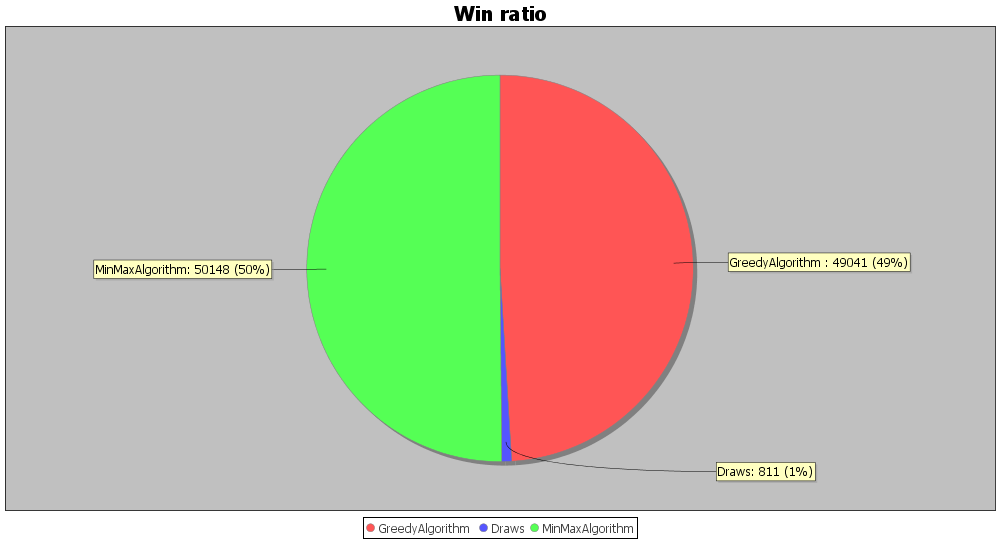
\includegraphics[width=\textwidth]{Resources/MirrorMmVsG/GVsMmWin.PNG}
	\caption{Wykres kołowy zwycięstw i remisów} 
	\label{fig:MirrorGVsMmWin}
\end{figure}

\begin{figure}[H]
	\centering
	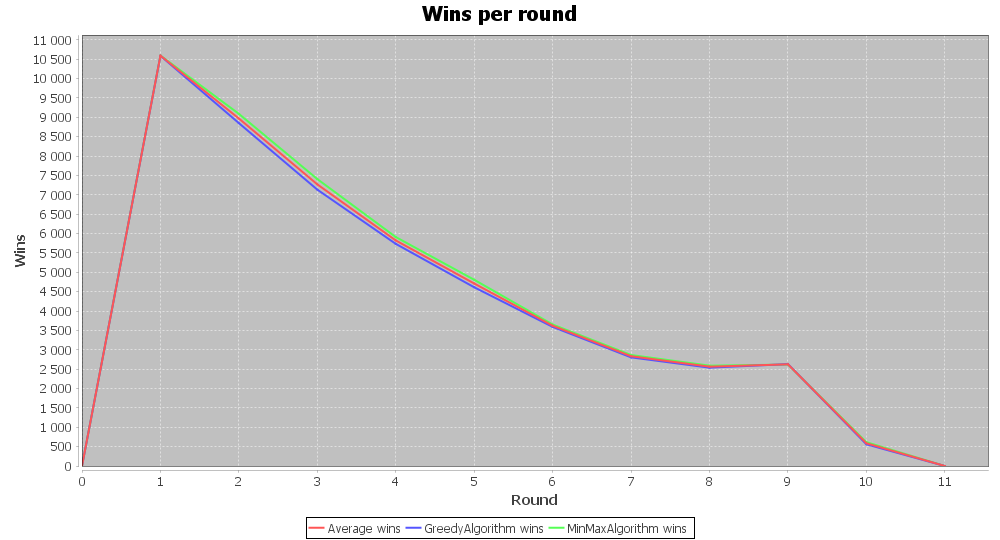
\includegraphics[width=\textwidth]{Resources/MirrorMmVsG/GVsMmRoundWin.PNG}
	\caption{Wykres wygranych w danej rundzie} 
	\label{fig:MirrorGVsMmRoundWin}
\end{figure}

Powyższe wykresy (rys. \ref{fig:MirrorGVsMmWin} i \ref{fig:MirrorGVsMmRoundWin}) pokazują niewielką przewagę algorytmu minimaksowego nad zachłannym, który w rundach od 1 do 8 zachowuje niewielką przewagę. W rundach 9 i 10 przeważa algorytm zachłanny, z czego wynika, że częściej wygrywa gry kończące się porównaniem siły kart.

\begin{figure}[H]
	\centering
	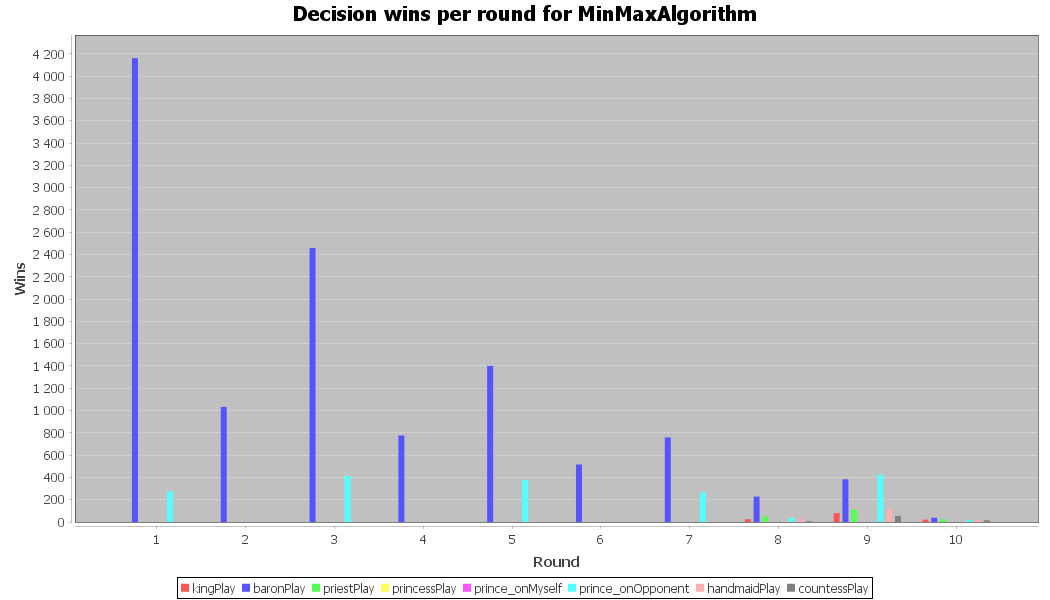
\includegraphics[width=\textwidth]{Resources/MirrorMmVsG/MmVsGDecision.PNG}
	\caption{Wykres zwycięskich zagrań} 
	\label{fig:MirrorMmVsGDecision}
\end{figure} 

\begin{figure}[H]
	\centering
	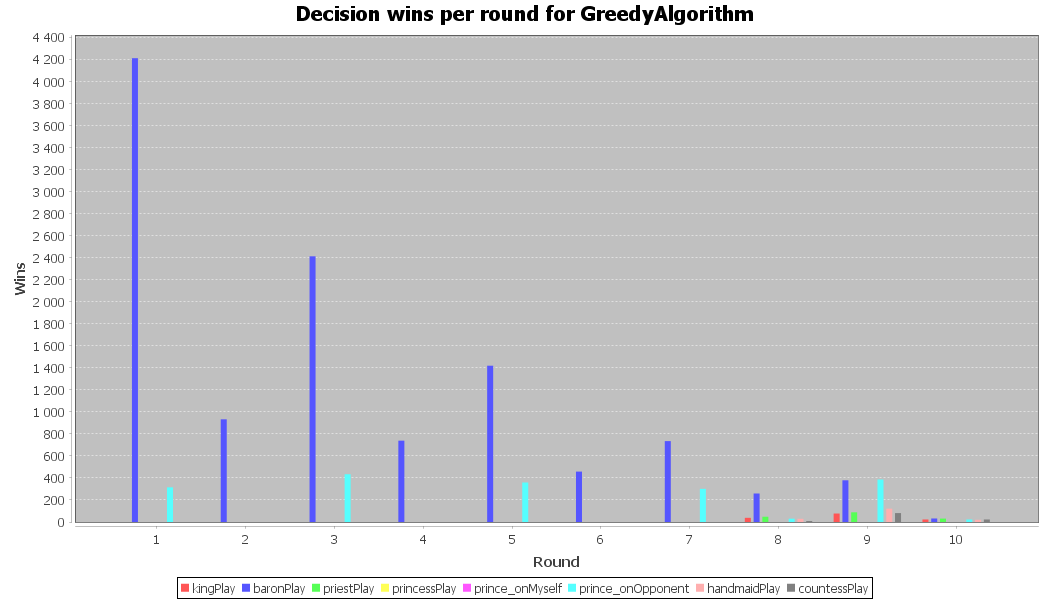
\includegraphics[width=\textwidth]{Resources/MirrorMmVsG/GVsMmDecision.PNG}
	\caption{Wykres zwycięskich zagrań} 
	\label{fig:MirrorGVsMmDecision}
\end{figure} 

\begin{figure}[H]
	\centering
	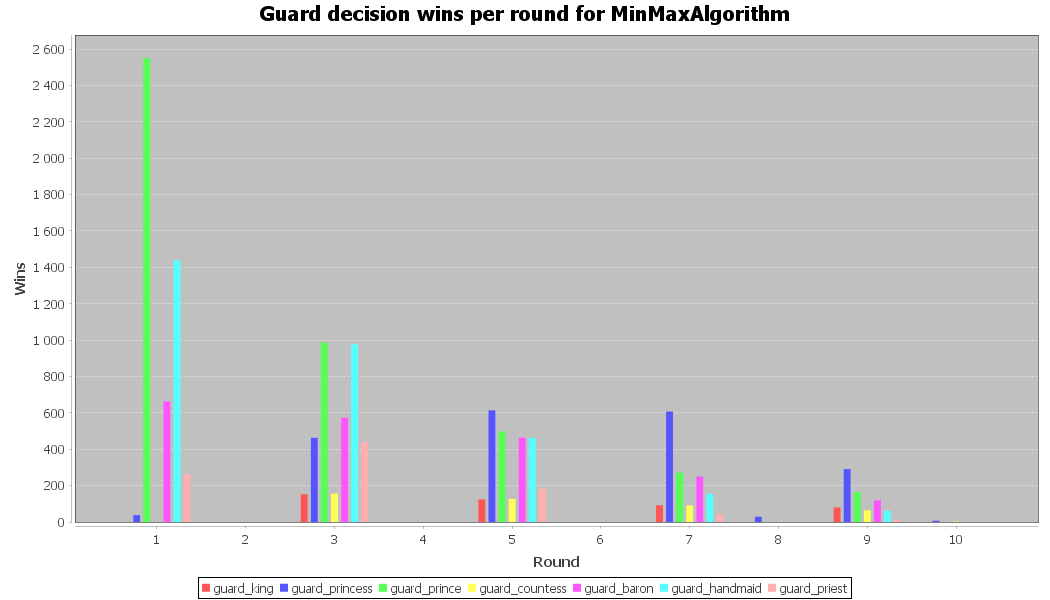
\includegraphics[width=\textwidth]{Resources/MirrorMmVsG/MmVsGGuardDecision.PNG}
	\caption{Wykres szczegółowy zwycięskich zagrań karty Strażniczki} 
	\label{fig:MmVsGGuardDecisionn}
\end{figure}

\begin{figure}[H]
	\centering
	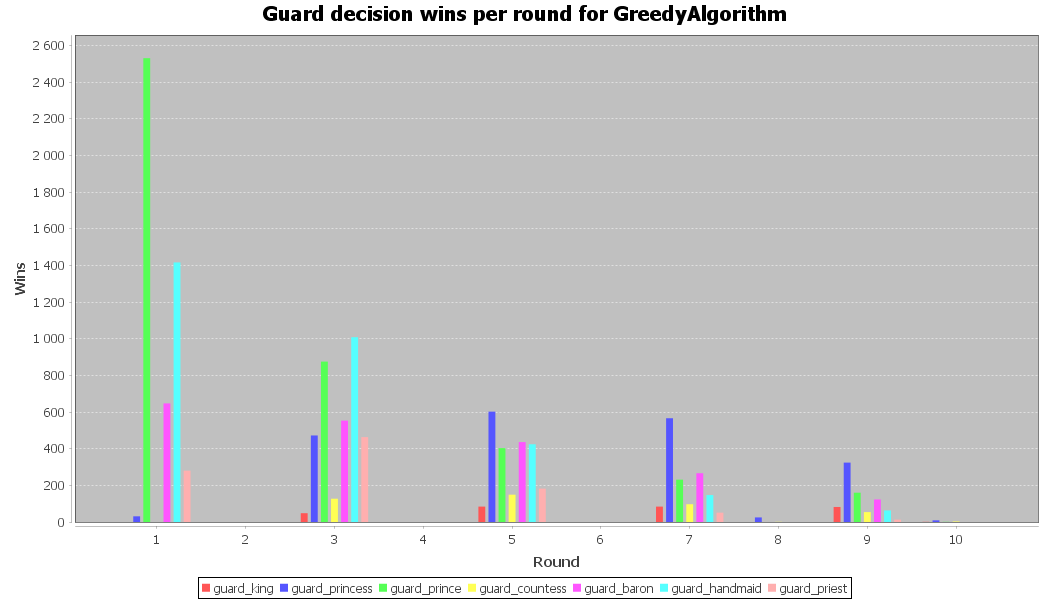
\includegraphics[width=\textwidth]{Resources/MirrorMmVsG/GVsMmGuardDecision.PNG}
	\caption{Wykres szczegółowy zwycięskich zagrań karty Strażniczki} 
	\label{fig:GVsMmGuardDecision}
\end{figure}


Oba algorytmy wykazują duże podobieństwa, a ewentualne różnice między nimi są takie same jak przy porównaniu z algorytmem losowym.
\clearpage
\section{Zachłanny versus MCTS}

\begin{figure}[H]
	\centering
	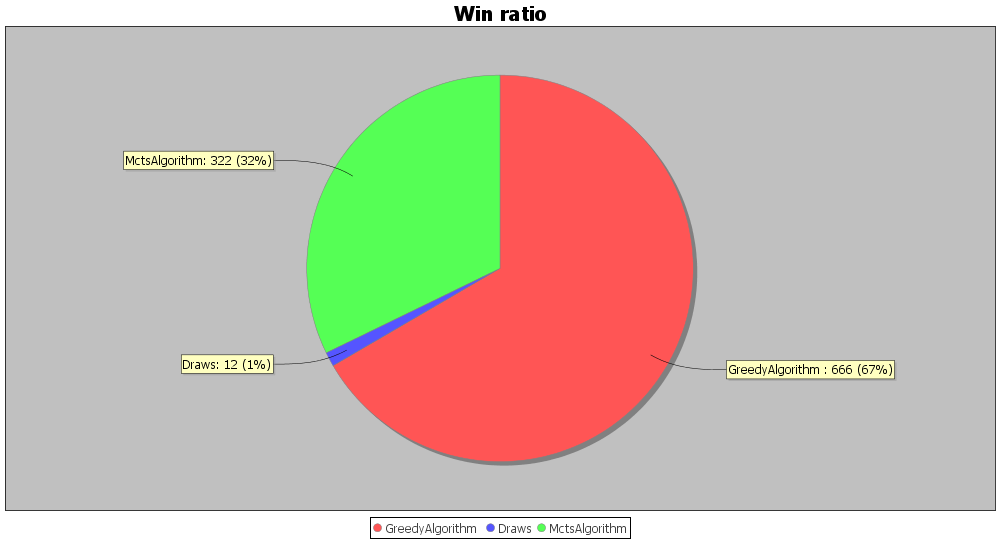
\includegraphics[width=\textwidth]{Resources/MirrorMctsVG/GVsMctsWin.PNG}
	\caption{Wykres kołowy zwycięstw i remisów} 
	\label{fig:GVsMctsWin}
\end{figure}

\begin{figure}[H]
	\centering
	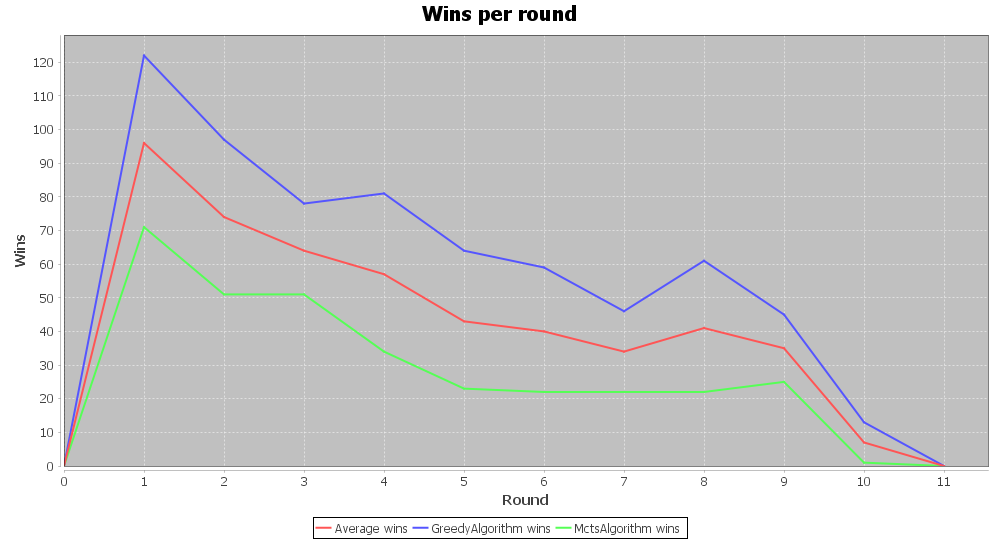
\includegraphics[width=\textwidth]{Resources/MirrorMctsVG/GVsMctsRoundWin.PNG}
	\caption{Wykres wygranych w danej rundzie} 
	\label{fig:GVsMctsRoundWin}
\end{figure}

Powyższe wykresy (rys. \ref{fig:GVsMctsWin} i \ref{fig:GVsMctsRoundWin}) pokazują bardzo wyraźną przewagę algorytmu zachłannego nad MCTS.

\begin{figure}[H]
	\centering
	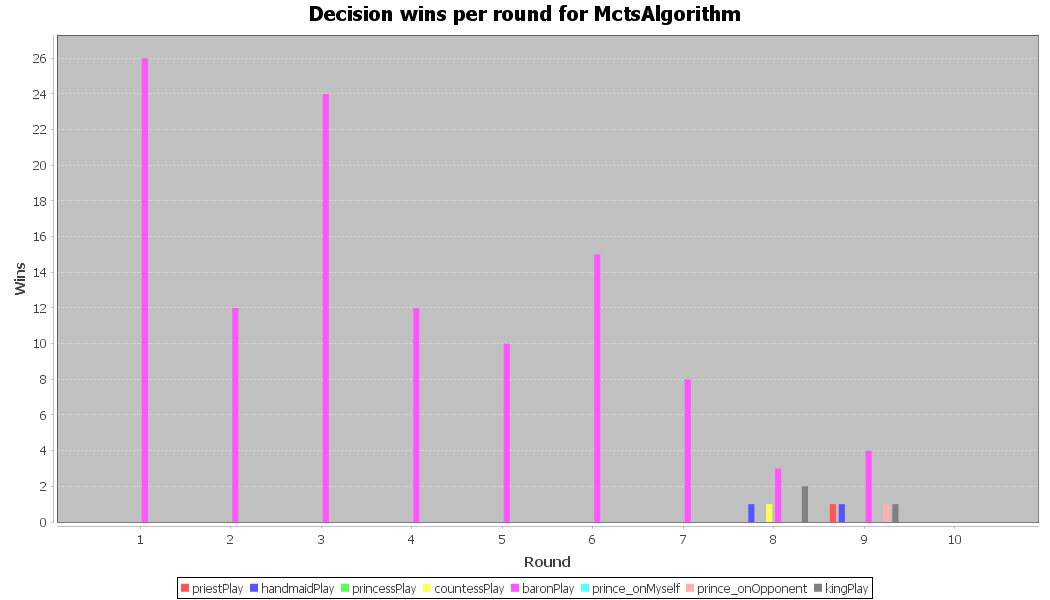
\includegraphics[width=\textwidth]{Resources/MirrorMctsVG/MctsVsGDecision.PNG}
	\caption{Wykres zwycięskich zagrań algorytmu MCTS} 
	\label{fig:MctsVsGDecision}
\end{figure} 

\begin{figure}[H]
	\centering
	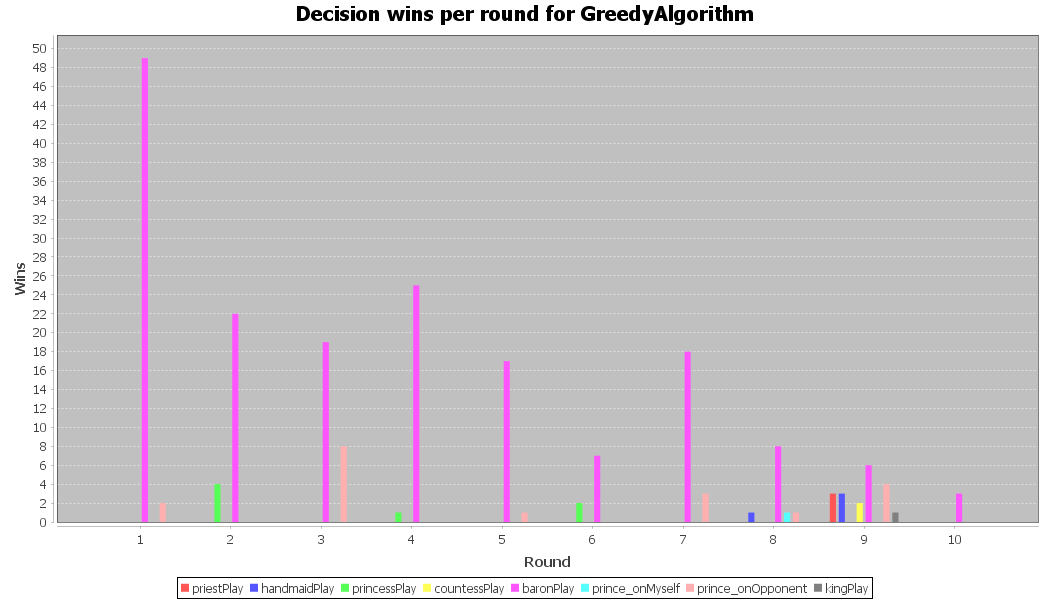
\includegraphics[width=\textwidth]{Resources/MirrorMctsVG/GVsMctsDecision.PNG}
	\caption{Wykres zwycięskich zagrań algorytmu zachłannego} 
	\label{fig:GVsMctsDecision}
\end{figure} 

Powyższe wykresy (rys. \ref{fig:MctsVsGDecision} i \ref{fig:GVsMctsDecision}) zwracają uwagę na nieregularność algorytmu MCTS do zwyciężania zagraniem karty Baron. Może to wynikać z tego, że MCTS częściej zatrzymuje w ręce kartę o wyższym numerze, i kiedy przeciwnik zagrywa kartę Barona, przegrywa.

\begin{figure}[H]
	\centering
	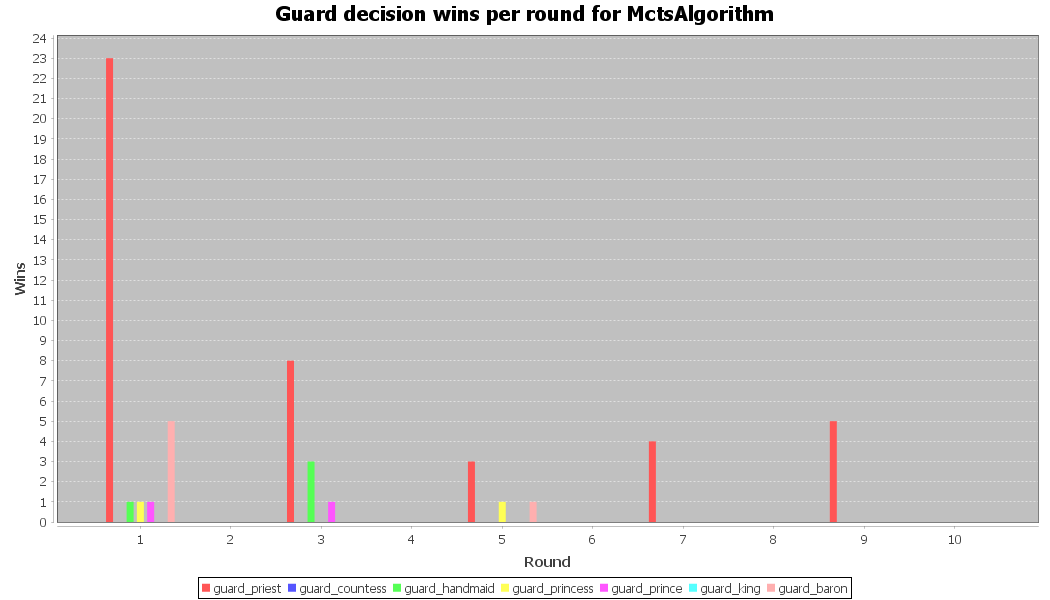
\includegraphics[width=\textwidth]{Resources/MirrorMctsVg/MctsVsGGuardDecision.PNG}
	\caption{Wykres szczegółowy zwycięskich zagrań karty Strażniczki} 
	\label{fig:MctsVsGGuardDecision}
\end{figure}

\begin{figure}[H]
	\centering
	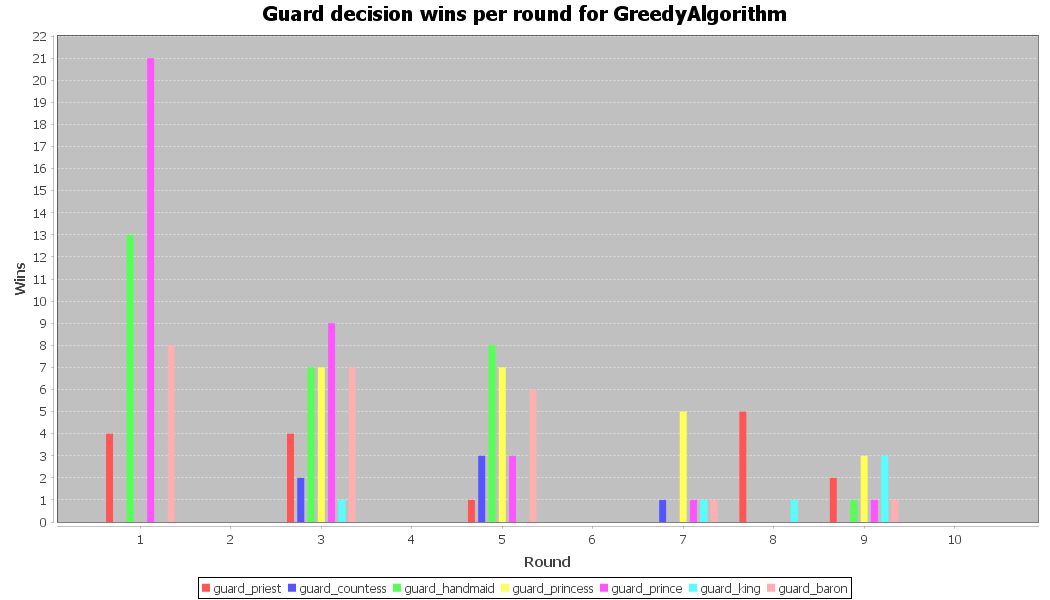
\includegraphics[width=\textwidth]{Resources/MirrorMctsVg/GVsMctsGuardDecision.PNG}
	\caption{Wykres szczegółowy zwycięskich zagrań karty Strażniczki} 
	\label{fig:GVsMctsGuardDecision}
\end{figure}

Na powyższych wykresach (rys. \ref{fig:MctsVsGGuardDecision} i \ref{fig:GVsMctsGuardDecision}) można zauważyć zupełnie inne tendencje do zagrywania karty Strażniczki. Algorytm MCTS niemal zawsze wybiera kartę Kapłana, natomiast algorytm zachłanny mimo że preferuje wybór Księcia, to niemal równie często wybiera inne typy kart.

\section{Minimaksowy versus MCTS}

\begin{figure}[H]
	\centering
	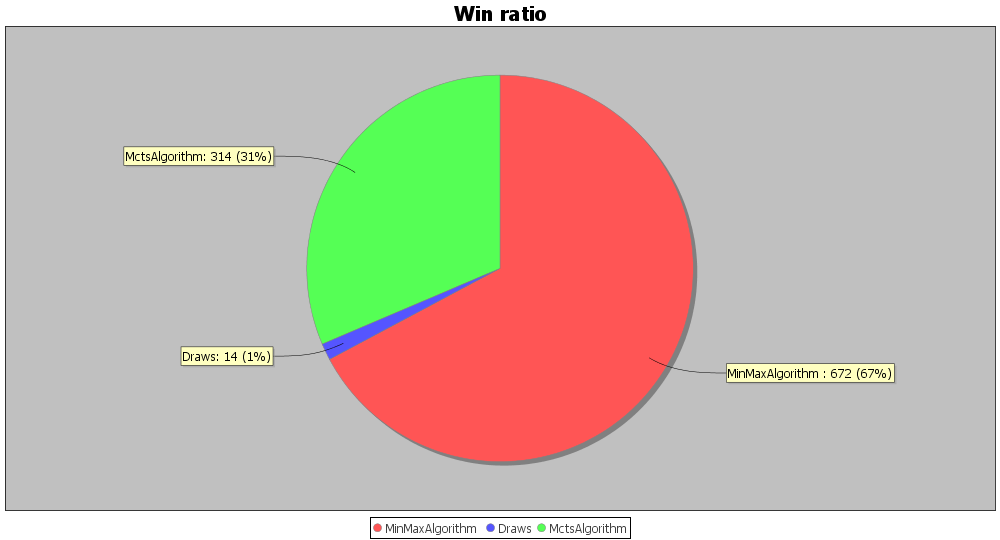
\includegraphics[width=\textwidth]{Resources/MirrorMmVsMcts/MmVsMctsWin.PNG}
	\caption{Wykres kołowy zwycięstw i remisów} 
	\label{fig:MmVsMctsWin}
\end{figure}

\begin{figure}[H]
	\centering
	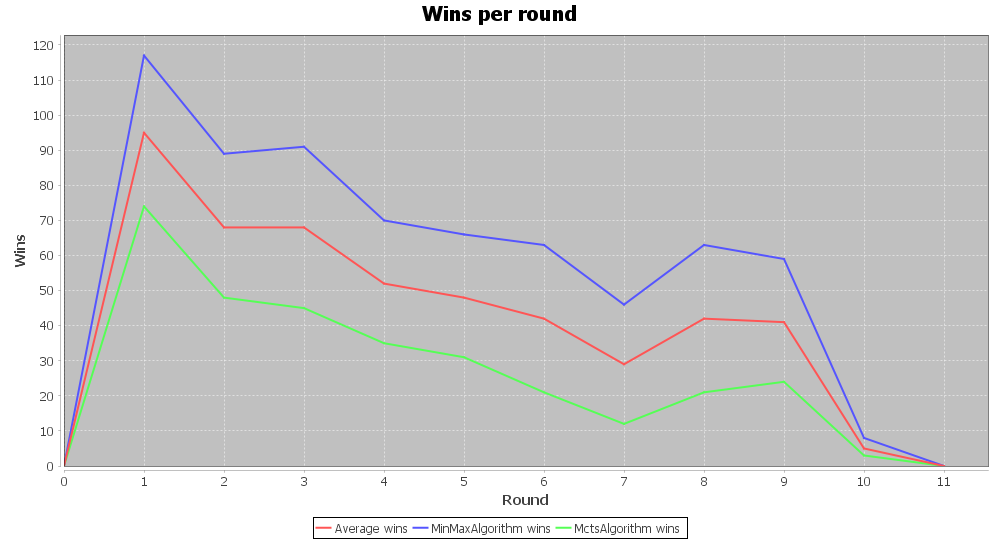
\includegraphics[width=\textwidth]{Resources/MirrorMmVsMcts/MmVsMctsRoundWin.PNG}
	\caption{Wykres wygranych w danej rundzie} 
	\label{fig:MmVsMctsRoundWin}
\end{figure}

Podobnie jak wcześniej, powyższe wykresy (rys. \ref{fig:MmVsMctsWin} i \ref{fig:MmVsMctsRoundWin}) pokazują przewagę algorytmu minimaksowego nad algorytmem MCTS.

\begin{figure}[H]
	\centering
	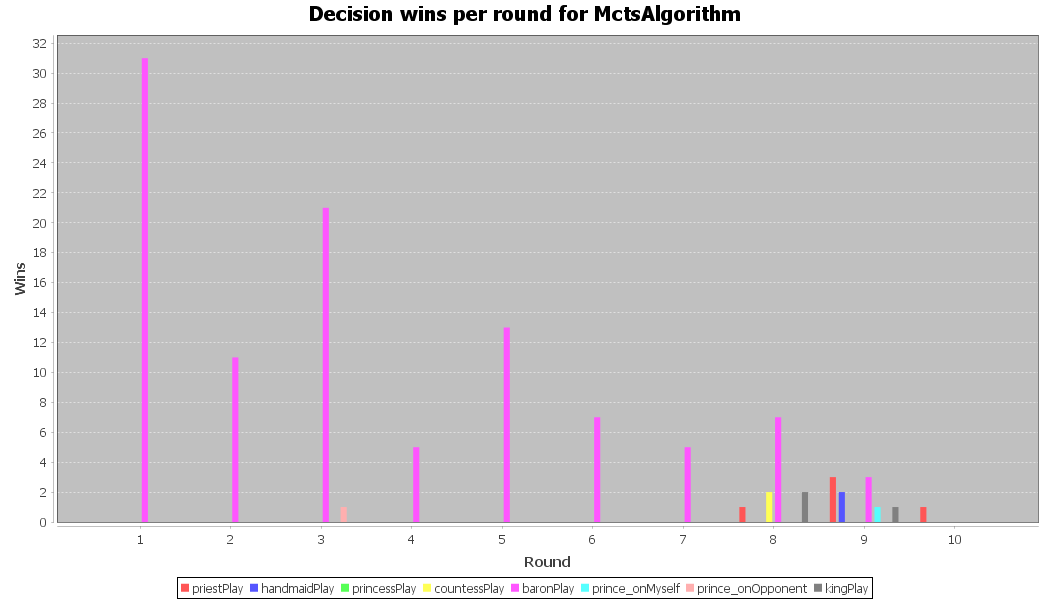
\includegraphics[width=\textwidth]{Resources/MirrorMmVsMcts/MctsVsMmDecision.PNG}
	\caption{Wykres zwycięskich zagrań algorytmu MCTS} 
	\label{fig:MctsVsMmDecision}
\end{figure} 

\begin{figure}[H]
	\centering
	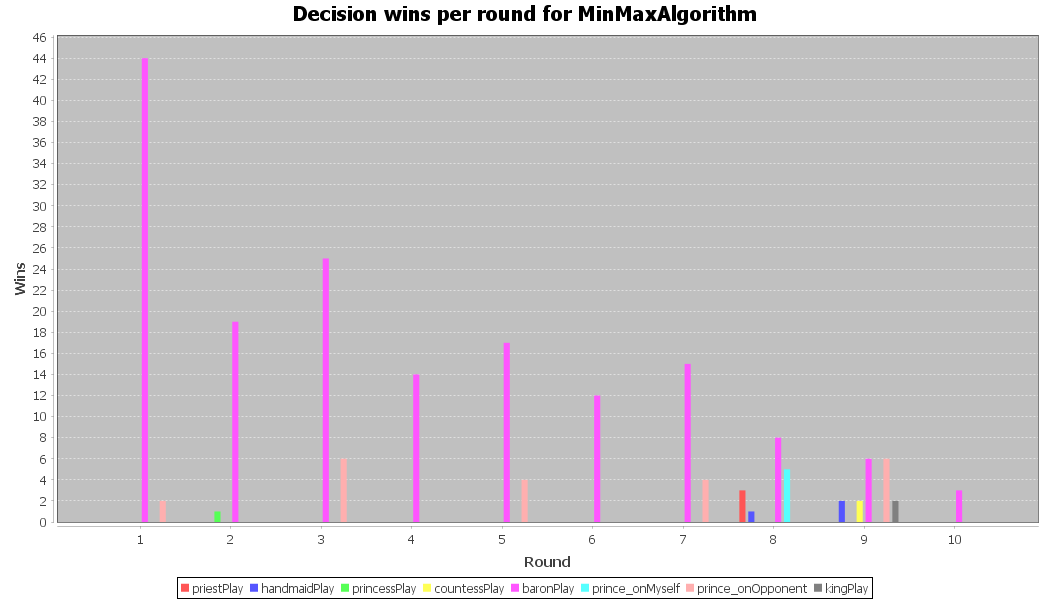
\includegraphics[width=\textwidth]{Resources/MirrorMmVsMcts/MmVsMctsDecision.PNG}
	\caption{Wykres zwycięskich zagrań algorytmu zachłannego} 
	\label{fig:MmVsMctsDecision}
\end{figure} 

Na powyższych wykresach (rys. \ref{fig:MctsVsMmDecision} warto zwrócić uwagę na statystykę zwycięskich zagrań w ostatnich rundach. Algorytm minimaksowy do końca zagrywa karty Barona i często wykorzystuje Księcia. Zwycięskie zagrania algorytmu MCTS w ostatnich rundach są bardziej równomiernie rozłożone, a w ostatniej rundzie nigdy nie zagrywa karty Barona.

\begin{figure}[H]
	\centering
	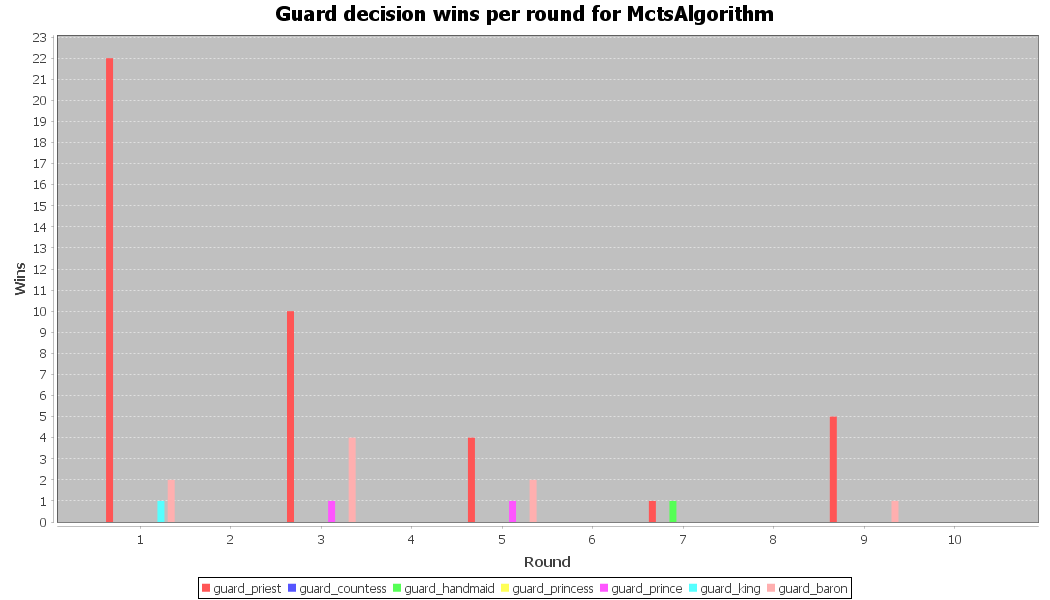
\includegraphics[width=\textwidth]{Resources/MirrorMmVsMcts/MctsVsMmGuardDecision.PNG}
	\caption{Wykres szczegółowy zwycięskich zagrań karty Strażniczki} 
	\label{fig:MctsVsMmGuardDecision}
\end{figure}

\begin{figure}[H]
	\centering
	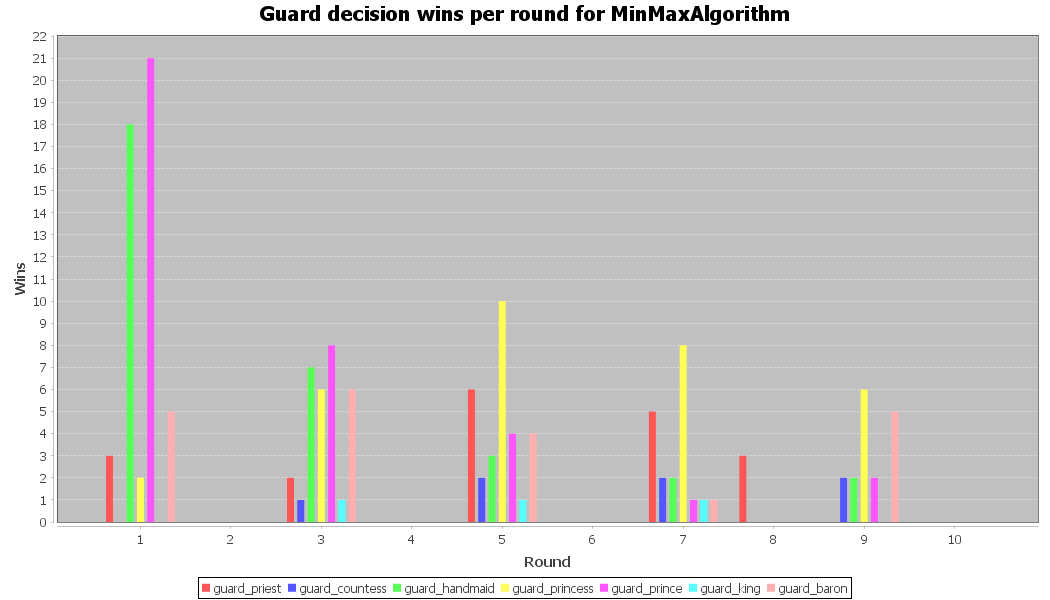
\includegraphics[width=\textwidth]{Resources/MirrorMmVsMcts/MmVsMctsGuardDecision.PNG}
	\caption{Wykres szczegółowy zwycięskich zagrań karty Strażniczki} 
	\label{fig:MmVsMctsGuardDecision}
\end{figure}

Na powyższych wykresach (rys. \ref{fig:MctsVsMmGuardDecision} i \ref{fig:MmVsMctsGuardDecision}) widać, że algorytm MCTS zachowuje się podobnie jak wcześniej. Natomiast algorytm minimaksowy zdecydowanie częściej zagrywa kartę Strażniczki z wyborem Księżniczki niż w było to w przypadku algorytmu zachłannego.

\section{Wnioski}
Zdecydowana większość gier kończy się w pierwszych 3 rundach, głównie poprzez zagranie kart Strażniczki i Barona. Wynika z tego również, że gracz rozpoczynający ma znaczną przewagę nad drugim graczem. W kolejnych rundach średnia ilość zwycięstw maleje, i następnie rośnie w dwóch ostatnich. Wynika to z dwóch zjawisk: po pierwsze, przy końcu gry gracze wyzbyli się już kart ofensywnych, czyli Strażniczki, Barona i Księcia, wobec czego dochodzi do porównania sił kart. Po drugie, jeśli karty ofensywne pozostały grze, znacznie wzrasta skuteczność ich użycia, co widać po częstości zagrań Strażniczki ze wskazaniem na Księżniczkę, bądź Księcia ze wskazaniem na przeciwnika (spodziewając się, że ma Księżniczkę). Ze statystyk można wywnioskować, że gra zdecydowanie sprzyja ofensywnym zagraniom.

Algorytm losowy nie wymaga głębokiej analizy - niemniej jednak warty uwagi jest fakt, że jest bardziej skuteczny niż algorytm MCTS.

Algorytm zachłanny osiąga wysokie wyniki w porównaniu z innymi algorytmami i niewiele niższe niż algorytm minimaksowy. Wynika to ze wspomnianego faworyzowania przez grę zagrań, które jak najszybciej zakończą grę. 

Algorytm minimaksowy osiąga wyniki tylko niewiele lepsze niż algorym zachłanny, pomimo znacznie dłuższego czasu działania. Warto pamiętać, że w przedstawionym wariancie dokonuje on tylko przeszukania drzewa rozwiązań do 1 ruchu w przód. Algorytm ten osiąga przewagę nad zachłannym w rundach środkowych, jednak różnica zwycięstw jest niewielka.

Monte Carlo Tree Search okazał się być największym rozczarowaniem, szczególnie, że jest mniej efektywny od algorytmu losowego. Przyczyną tego stanu rzeczy jest moje błędne założenie, że negatywny wpływ elementu losowego na algorytm może zostać zniwelowany przez ilość symulacji przeprowadzanych przez MCTS. Niestety, implementacja algorytmu w formie podstawowej sprawia, że wpada on w pewną pułapkę już podczas pierwszego kroku. Wynika to z tego, że gracz w danym momencie gry nie zna całego jej stanu, lecz zbiór informacyjny \textit{I}, w związku z tym w korzeniu drzewa zawarty jest jeden wylosowany stan z tego zbioru informacyjnego. Biorąc pod uwagę ilość stanów w tym zbiorze, szansa, że zostanie wylosowany ten faktyczny, jest niewielka. Każda symulacja wykonana na błędnie założonym stanie początkowym w korzeniu drzewa algorytmu MCTS będzie prowadzić do błędnych wniosków. W efekcie MCTS osiąga gorsze wyniki niż algorytm losowy. Można by to podsumować potocznym stwierdzeniem, że "lepszy jest brak wiedzy niż wiedza nieprawdziwa".